

\section{Procedure}

So far, the problem has been introduced and the required terminology has been defined. In the procedure section,
 the details of {\sc ModifiedSJT} and {\sc CyclicBar} are provided. These details include the pseudocode for 
 each of the algorithms, the initial conditions for each of the algorithms, the structures produced by each 
 of the algorithms, and a number of lemmas and proofs for each of the two algorithms. In the procedure section, 
 the algorithms are assessed independently of each other.
%%section SJT
\subsection{The Modified Steinhaus-Johnson-Trotter Algorithm}

For the initial conditions of {\sc ModifiedSJT} assume the following. 
Let be the $ladder$ be initialized a two dimensional binary array of only $0's$.
 Let a $1$ at $row=i,col=j$ 
indicate a bar at  $row=i,col=j$. Let a $0$ at $row=i,col=j$ 
indicate the absence of a bar at  $row=i,col=j$.
Let $n$ be the maximum element. Let $direction$ be a one 
indexed array set to left for all indexes. Let left indicate that a bar is to be added to the ladder; bars 
are added left to right. Let right indicate a bar is to be removed from the ladder; bars 
are removed right to left. Let $route$ be initialized to $2$. On each recursive call 
$route$ is incremented by $1$ from $2,3 \dots n$.
\begin{algorithm}
  \begin{algorithmic}[1]
    \Function{ModifiedSJT}{$n$, $ladder$, $route$, $direction$}
     %%base case
      \If{$route > n$}
        \State {\sc print}($ladder$)
        \State \textbf{return}
      \EndIf
      %%swap the nth element n-1 times
      \For{$i$ \textbf{from} $0$ \textbf{to} $route-1$}
        \If{$i = 0$}
          \State {\sc ModifiedSJT}($n$, $ladder$, $route+1$, $direction$)
        \Else 
          \If{$direction[route]=$ left}
            \State $row \gets (n) + (n - route) - (i);$
            \State $col \gets route - i$
            \State $ladder[row][col] \gets 1$
          \Else
            \State $col \gets i$
            \State $row \gets 2(n - route) + (i)$
            \State $ladder[row][col] \gets 0$
          \EndIf
        \EndIf
        \State {\sc ModifiedSJT}($n$, $ladder$, $route+1$, $direction$)
      \EndFor
      \If{$direction[route] =$ left}
        \State $direction[route] \gets$ right
      \Else
        \State $direction[route] \gets$ left
      \EndIf
    \EndFunction
  \end{algorithmic}
  \caption{Modification of the {\sc SJT} algorithm for listing $L_{n}$}
  \label{Alg:ModSJT}
\end{algorithm}


\pagebreak


The principles of the algorithm are the following. Given $route=k$, add or remove a bar for route $k$, then add or remove 
all bars for $route=k+1$. Once all bars for route $k+1$ have been added or removed, 
proceed to add or remove the next bar from $route=k$. Repeat until all $k-1$ bars have been added or removed from route $k$.
If $direction[route]$ is left, then bars of $route$ will be added to 
$ladder$ from right to left, bottom to top, until no more bars to $route$ can be added.
If $direction[route]$ is right, then bars will be removed from $ladder$, right to left, top to bottom, until 
no more bars from $route$ can be removed. Once all the bars for $route$ have 
been added or removed, then $direction[route]$ is reversed,
indicating that the opposite operation will be applied to the bars of the route when 
$route$ is next processed. The maximum number of bars for a given $route=k$ is $k-1$ and the minimum number of 
bars is $1$. On each recursive call, $route$ is 
incremented by $1$. When $route$ is greater than $n$, print the ladder 
and return. 


\begin{lemma}
  {\sc ModifiedSJT} produces $L_{n}$
\end{lemma}
\begin{proof}
  Since the algorithm is a modification of the Steinhaus-Johnson-Trotter algorithm, a similar proof for the SJT algorithm 
can be applied to the {\sc ModifiedSJT} algorithm. Suppose we want to list all $n!$ ladders 
of order $n$. Suppose we have all $n-1!$ ladders of order $n-1$, then for 
each ladder of order $n-1$ add a new column to the right; this results in $n-1$ columns seeing as 
the number of columns is one less than the number of elements. For each of the $n-1!$ ladders with $n-1$ columns 
add $0 \dots n-1$ bars beginning at column $n-1$ and ending 
at column $1$. Doing so results in $(n-1)!n=n!$ ladders of order $n$. To see 
an example of the proof please refer to Figure~\ref{Fig:CanLSJT}.
\end{proof}
%%prove the dimensions of the datastructure
\begin{center}
 \begin{figure}[!htp]
  \centering
  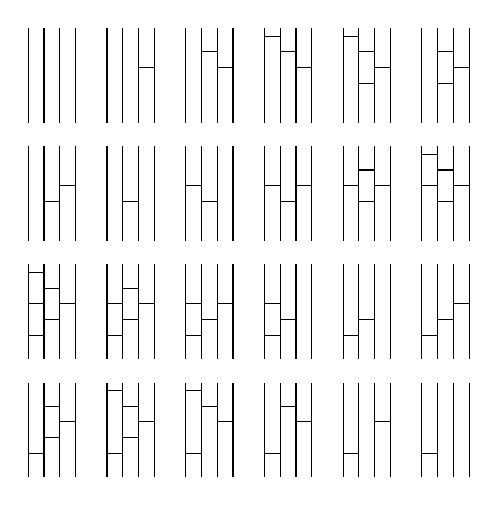
\begin{tikzpicture}
\draw(0.00,5.90) to (0.00,7.10);
\draw(0.20,5.90) to (0.20,7.10);
\draw(0.40,5.90) to (0.40,7.10);
\draw(0.60,5.90) to (0.60,7.10);


\draw(1.00,5.90) to (1.00,7.10);
\draw(1.20,5.90) to (1.20,7.10);
\draw(1.40,5.90) to (1.40,7.10);
\draw(1.60,5.90) to (1.60,7.10);
\draw(1.40, 6.60) to (1.60, 6.60);


\draw(2.00,5.90) to (2.00,7.10);
\draw(2.20,5.90) to (2.20,7.10);
\draw(2.40,5.90) to (2.40,7.10);
\draw(2.60,5.90) to (2.60,7.10);
\draw(2.20, 6.80) to (2.40, 6.80);
\draw(2.40, 6.60) to (2.60, 6.60);


\draw(3.00,5.90) to (3.00,7.10);
\draw(3.20,5.90) to (3.20,7.10);
\draw(3.40,5.90) to (3.40,7.10);
\draw(3.60,5.90) to (3.60,7.10);
\draw(3.00, 7.00) to (3.20, 7.00);
\draw(3.20, 6.80) to (3.40, 6.80);
\draw(3.40, 6.60) to (3.60, 6.60);


\draw(4.00,5.90) to (4.00,7.10);
\draw(4.20,5.90) to (4.20,7.10);
\draw(4.40,5.90) to (4.40,7.10);
\draw(4.60,5.90) to (4.60,7.10);
\draw(4.00, 7.00) to (4.20, 7.00);
\draw(4.20, 6.80) to (4.40, 6.80);
\draw(4.40, 6.60) to (4.60, 6.60);
\draw(4.20, 6.40) to (4.40, 6.40);


\draw(5.00,5.90) to (5.00,7.10);
\draw(5.20,5.90) to (5.20,7.10);
\draw(5.40,5.90) to (5.40,7.10);
\draw(5.60,5.90) to (5.60,7.10);
\draw(5.20, 6.80) to (5.40, 6.80);
\draw(5.40, 6.60) to (5.60, 6.60);
\draw(5.20, 6.40) to (5.40, 6.40);


\draw(0.00,4.40) to (0.00,5.60);
\draw(0.20,4.40) to (0.20,5.60);
\draw(0.40,4.40) to (0.40,5.60);
\draw(0.60,4.40) to (0.60,5.60);
\draw(0.40, 5.10) to (0.60, 5.10);
\draw(0.20, 4.90) to (0.40, 4.90);


\draw(1.00,4.40) to (1.00,5.60);
\draw(1.20,4.40) to (1.20,5.60);
\draw(1.40,4.40) to (1.40,5.60);
\draw(1.60,4.40) to (1.60,5.60);
\draw(1.20, 4.90) to (1.40, 4.90);


\draw(2.00,4.40) to (2.00,5.60);
\draw(2.20,4.40) to (2.20,5.60);
\draw(2.40,4.40) to (2.40,5.60);
\draw(2.60,4.40) to (2.60,5.60);
\draw(2.00, 5.10) to (2.20, 5.10);
\draw(2.20, 4.90) to (2.40, 4.90);


\draw(3.00,4.40) to (3.00,5.60);
\draw(3.20,4.40) to (3.20,5.60);
\draw(3.40,4.40) to (3.40,5.60);
\draw(3.60,4.40) to (3.60,5.60);
\draw(3.00, 5.10) to (3.20, 5.10);
\draw(3.40, 5.10) to (3.60, 5.10);
\draw(3.20, 4.90) to (3.40, 4.90);


\draw(4.00,4.40) to (4.00,5.60);
\draw(4.20,4.40) to (4.20,5.60);
\draw(4.40,4.40) to (4.40,5.60);
\draw(4.60,4.40) to (4.60,5.60);
\draw(4.20, 5.30) to (4.40, 5.30);
\draw(4.00, 5.10) to (4.20, 5.10);
\draw(4.40, 5.10) to (4.60, 5.10);
\draw(4.20, 4.90) to (4.40, 4.90);


\draw(5.00,4.40) to (5.00,5.60);
\draw(5.20,4.40) to (5.20,5.60);
\draw(5.40,4.40) to (5.40,5.60);
\draw(5.60,4.40) to (5.60,5.60);
\draw(5.00, 5.50) to (5.20, 5.50);
\draw(5.20, 5.30) to (5.40, 5.30);
\draw(5.00, 5.10) to (5.20, 5.10);
\draw(5.40, 5.10) to (5.60, 5.10);
\draw(5.20, 4.90) to (5.40, 4.90);


\draw(0.00,2.90) to (0.00,4.10);
\draw(0.20,2.90) to (0.20,4.10);
\draw(0.40,2.90) to (0.40,4.10);
\draw(0.60,2.90) to (0.60,4.10);
\draw(0.00, 4.00) to (0.20, 4.00);
\draw(0.20, 3.80) to (0.40, 3.80);
\draw(0.00, 3.60) to (0.20, 3.60);
\draw(0.40, 3.60) to (0.60, 3.60);
\draw(0.20, 3.40) to (0.40, 3.40);
\draw(0.00, 3.20) to (0.20, 3.20);


\draw(1.00,2.90) to (1.00,4.10);
\draw(1.20,2.90) to (1.20,4.10);
\draw(1.40,2.90) to (1.40,4.10);
\draw(1.60,2.90) to (1.60,4.10);
\draw(1.20, 3.80) to (1.40, 3.80);
\draw(1.00, 3.60) to (1.20, 3.60);
\draw(1.40, 3.60) to (1.60, 3.60);
\draw(1.20, 3.40) to (1.40, 3.40);
\draw(1.00, 3.20) to (1.20, 3.20);


\draw(2.00,2.90) to (2.00,4.10);
\draw(2.20,2.90) to (2.20,4.10);
\draw(2.40,2.90) to (2.40,4.10);
\draw(2.60,2.90) to (2.60,4.10);
\draw(2.00, 3.60) to (2.20, 3.60);
\draw(2.40, 3.60) to (2.60, 3.60);
\draw(2.20, 3.40) to (2.40, 3.40);
\draw(2.00, 3.20) to (2.20, 3.20);


\draw(3.00,2.90) to (3.00,4.10);
\draw(3.20,2.90) to (3.20,4.10);
\draw(3.40,2.90) to (3.40,4.10);
\draw(3.60,2.90) to (3.60,4.10);
\draw(3.00, 3.60) to (3.20, 3.60);
\draw(3.20, 3.40) to (3.40, 3.40);
\draw(3.00, 3.20) to (3.20, 3.20);


\draw(4.00,2.90) to (4.00,4.10);
\draw(4.20,2.90) to (4.20,4.10);
\draw(4.40,2.90) to (4.40,4.10);
\draw(4.60,2.90) to (4.60,4.10);
\draw(4.20, 3.40) to (4.40, 3.40);
\draw(4.00, 3.20) to (4.20, 3.20);


\draw(5.00,2.90) to (5.00,4.10);
\draw(5.20,2.90) to (5.20,4.10);
\draw(5.40,2.90) to (5.40,4.10);
\draw(5.60,2.90) to (5.60,4.10);
\draw(5.40, 3.60) to (5.60, 3.60);
\draw(5.20, 3.40) to (5.40, 3.40);
\draw(5.00, 3.20) to (5.20, 3.20);


\draw(0.00,1.40) to (0.00,2.60);
\draw(0.20,1.40) to (0.20,2.60);
\draw(0.40,1.40) to (0.40,2.60);
\draw(0.60,1.40) to (0.60,2.60);
\draw(0.20, 2.30) to (0.40, 2.30);
\draw(0.40, 2.10) to (0.60, 2.10);
\draw(0.20, 1.90) to (0.40, 1.90);
\draw(0.00, 1.70) to (0.20, 1.70);


\draw(1.00,1.40) to (1.00,2.60);
\draw(1.20,1.40) to (1.20,2.60);
\draw(1.40,1.40) to (1.40,2.60);
\draw(1.60,1.40) to (1.60,2.60);
\draw(1.00, 2.50) to (1.20, 2.50);
\draw(1.20, 2.30) to (1.40, 2.30);
\draw(1.40, 2.10) to (1.60, 2.10);
\draw(1.20, 1.90) to (1.40, 1.90);
\draw(1.00, 1.70) to (1.20, 1.70);


\draw(2.00,1.40) to (2.00,2.60);
\draw(2.20,1.40) to (2.20,2.60);
\draw(2.40,1.40) to (2.40,2.60);
\draw(2.60,1.40) to (2.60,2.60);
\draw(2.00, 2.50) to (2.20, 2.50);
\draw(2.20, 2.30) to (2.40, 2.30);
\draw(2.40, 2.10) to (2.60, 2.10);
\draw(2.00, 1.70) to (2.20, 1.70);


\draw(3.00,1.40) to (3.00,2.60);
\draw(3.20,1.40) to (3.20,2.60);
\draw(3.40,1.40) to (3.40,2.60);
\draw(3.60,1.40) to (3.60,2.60);
\draw(3.20, 2.30) to (3.40, 2.30);
\draw(3.40, 2.10) to (3.60, 2.10);
\draw(3.00, 1.70) to (3.20, 1.70);


\draw(4.00,1.40) to (4.00,2.60);
\draw(4.20,1.40) to (4.20,2.60);
\draw(4.40,1.40) to (4.40,2.60);
\draw(4.60,1.40) to (4.60,2.60);
\draw(4.40, 2.10) to (4.60, 2.10);
\draw(4.00, 1.70) to (4.20, 1.70);


\draw(5.00,1.40) to (5.00,2.60);
\draw(5.20,1.40) to (5.20,2.60);
\draw(5.40,1.40) to (5.40,2.60);
\draw(5.60,1.40) to (5.60,2.60);
\draw(5.00, 1.70) to (5.20, 1.70);






\end{tikzpicture}
  \caption{$L_{4}$ generated by the {\sc ModifiedSJT} algorithm. The algorithm inserts or removes a bar between any two successive ladders.}
  \label{Fig:CanLSJT}
\end{figure}
\end{center}\pagebreak

\begin{theorem}
  If the algorithm being applied is {\sc ModifiedSJT} then the number of rows required for the ladder data-structure is $2(n-1) - 1$ 
  and the number of columns required for the ladder is $n-1$.
\end{theorem}
\begin{proof}
  The number of columns is fairly straightforward. Seeing as there are always $n$ elements in $\pi_{n}$, 
  a column represents a gap between lines in the corresponding ladder lottery. Each ladder of order $n$ has $n$ lines, 
  one for each element in $\pi_{n}$. Therefore each ladder of order $n$ has $n-1$ columns.\par 
  The number of rows for the ladder data-structure is calculated a follows, given $\pi_{n}$, the minimal 
  number of rows required is when $\pi_{n}$ is sorted. In this case there are zero rows because there are 
  zero bars added to the ladder. When a bar is added to the ladder it can be added to an already existing row 
  or to a new row. If the current state of the ladder is empty then adding the first bar produces the second ladder in
  $L_{n}$. Since the bars are being added bottom right to top left, and the first bar to be added belongs 
  to the $nth$ route, then it must be added to $row=n-1$, $col=n-1$. As bars of the $nth$ route get 
  continuously added to the ladder, each bar is added a row above the previous bar and to a column 
  to the left of the column of the previous bar.
  Since no two bars of the $nth$ route can be on the same row, this will require $n-1$ rows. Note, if they were added to the same 
  row, then the left end point of the right bar would be touching the right end point of the left bar which is disallowed. Once the 
  bars of the $nth$ element are added, the bars of the $n-1th$ route will be added. The $n-1th's$ first bar 
  will be added to the $n-2$ column, otherwise it would be directly below the first bar of the $nth$ route, which is a violation. 
  Since the first bar of the $n-1$'s element is added to column $n-2$, then it must be given a new row, otherwise its right end point 
  will be touching  the left end point of the first bar of route $n$. The remaining $n-2$ bars of element $n-1$
  will be added bottom right to top left, but none of their end points will touch the end points of element $n$ seeing as they will 
  always be two columns apart from any bar in $n's$ route. The same logic applies to element $n-2$, it will require one extra row for its 
  first bar, in order not to touch the first bar of element $n-1$, but the remainder of its bars will always be two columns away from 
  the remainder of the bars for $n-1$, etc. Therefore there are $n-1$ rows required for the $nth$ element and each subsequent 
  element, $k$ requires only one new row. Since $2 \leq k < n$, then there are $(n-2)$ additional rows required for the ladder. Note that element 
  $1$ has no bars in its route. Therefore there are $(n-1)$ rows required for element $n's$ bars  plus $(n-2)$ rows required for 
  all the remaining $2 \leq k < n$ routes. In conclusion the number of rows required is $(n-1) + (n-2) = 2(n-1)-1$. 
  See figure for the tree of ladders 
  generated by {\sc ModifiedSJT} for $n=4$. Note that the maximum number of rows required is $2(n-1)-1=2(3)-1=5$.
\end{proof}



%%end proof
From looking at Figure~\ref{Fig:CanLSJT} it should be clear that the canonical representative from $L_{n}$ when using the 
{\sc ModifiedSJT} algorithm is also the root ladder from each $OptL\{\pi\}$. Recall that the root ladder is the 
ladder whose bars of a lesser route have not crossed the bars of a greater route. In the case of the 
{\sc ModifiedSJT} algorithm, transitioning from one ladder to the next involves simply inserting a new bar 
or removing a bar. Let $k$ be the current route. If a new bar being added belongs to 
route $k$, the bar is added below the route of $k+1$ and above the route of $k-1$, therefore 
adding a bar does not violate the constraint of the root ladder. Let $l_{i}$ be the current ladder.
Let $l_{i+1}$ be the next ladder in the sequence. 
Then removing a bar from $l_{i}$ cannot make $l_{i+1}$ a non-root ladder, because 
removing a bar from $l_{i}$ does not allow the bar of a lesser element to cross the bars of a greater element.
Thus, the canonical representative for $L_{n}$ is always the root ladder from each $OptL\{\pi\}$.\par 



%%Beging the cases
The calculations for the row and column for the bar 
depend on whether the bar is being added or removed. Thus, there are
four cases to consider. The cases are the following: 
\begin{caseof}
 ~\case{Bar is being added}{Row is being calculated.}
 ~\case{Bar is being added}{Column is being calculated.}
 ~\case{Bar is being removed}{Row is being calculated.}
 ~\case{Bar is being removed.}{Column is being calculated.}
\end{caseof}

%%End the cases

%%proof 1
\begin{lemma}
  Assume a bar is being added. Let $i$ be the current number of bars in the ladder for $route=k[2 \dots n]$.
  Then the $row=(n-1)+(n-route)-i$.
\end{lemma}
\begin{proof}
   It must be noted that we are listing only root ladders. So when transitioning from 
$l_{j}$ to $l_{j+1}$ in $L_{n}$ both are root ladders. With this in mind, one can say that the 
number of rows required for $route=n$ is $n-1$ seeing as the $nth$ value can have at most $n-1$ bars in its route, 
each requiring  their own 
row. Thus, the $(n-1)$ term in the equation in included for the $n-1$ bars of 
$route=n$. The $(n-route)$ term is added to $(n-1)$ indicating 
an offset value for the first bar of the $route$; this term calculates 
the difference in rows between the first bar of $route=n$ 
and the first bar of $route=k$. If $route=n$ 
then $offset=0$, if $route=n-1$ then $offset=1$, if $route=n-2$ then $offset=2$, etc.
Since bars are added right to left, bottom, up, then the first bar of $route=k$ will be added 
at $row=(n-1)+(n-route)$. When a bar is added to $route=k$ route, the $i$ value is incremented by one. This value is subtracted in 
order to effectively move up the ladder as bars are added to $route=k$. Since bars are added 
bottom to top, $row$ needs to be decremented for each new bar to be added. Refer to Figure~\ref{Fig:SJTcase1} for an example of 
row calculation when adding a bar.
\end{proof}
\begin{figure}[!htp]
  \begin{center}
    
    \begin{tikzpicture}

    \draw(0, -2) to (0, 6);
       \draw(0, 5.5) to (2, 5.5);
       \node at (1, 5.7){5,1};
       \node at (-1, 5.5){R1};
     \draw(2, -2) to (2, 6);
       \draw(2, 4.5) to (4, 4.5);
       \draw(2, 0.5) to (4, 0.5);
       \node at (3, 4.7){5,3};
       \node at(3, 0.7){3, 2};
       \node at(-1, 4.5){R2};
     \draw(4, -2) to (4, 6);
       \draw(4, 3.5) to (6, 3.5);
       \node at(5, 3.7){5,2};
       \node at(-1, 3.5){R3};
     \draw(6, -2) to (6, 6);
       \draw(6, 2.5) to (8, 2.5);
       \node at(7, 2.7){5,4};
       \node at(-1, 2.5){R4};
     \draw(8, -2) to (8, 6);

    \node at(-1, 1.5){R5};
    \node at(-1, 0.5){R6};
    \node at(-1, -0.5){R7};
    \draw (1,1.5) ellipse (1cm and .4cm);

  \end{tikzpicture}

\end{center}
\caption{The second bar of route 3 goes will go in row 5, column 1. $5 = (5-1)+(5-3)-1 = (n-1)+(n-route)-i$.}
\label{Fig:SJTcase1}
\end{figure}
\pagebreak
%%end proof 1


%%Prove case 2
\begin{lemma}
  Assume a bar is being added. Let $i$ be the current number of bars in the ladder for $route=k[2 \dots n]$.
  Then the $col=route-1-i$.
\end{lemma}
\begin{proof}
  The total number of bars required for $route=k$ is $k-1$, each requiring their own column. The columns 
  span from $1 \dots k-1$. The 
  bars are added right to left and when a bar is added $i$ is incremented by one. 
  Since bars are 
  added right to left, the first bar 
  of $route=k$ is inserted at column $k-1$. This is because the first bar of the $kth$ route is the left child bar of the 
  lowest bar of the $k+1th$ route. Let $y$ be the first bar to be added for $route=k$ and let $x$ be 
  the 
  lowest bar of the $route=k+1$. $x$ is the parent bar of $y$ and $y$ is the left child of 
  $x$ for the following reasons. If $y$ was directly below $x$, then the ladder would have redundant bars, thus making it 
  non-optimal. If $y$ was to the right of $x$, then $y$ would either be above $x$, thus violating the property of the root ladder, 
  or if $y$ were below $x$ and to the right of $x$ then $y$ would be part of the route for $k+1$, yet this is a contradiction 
  seeing as we said $y$ belongs to $k's$ route. Therefore, $y$ must be in a column to the left of $x$. As bars are added 
  to $k's$ route, $i$ is incremented for each bar. $i$ is subtracted from the original column, $k-1$, effectively moving 
  to the next column to the left in $ladder$. See Figure~\ref{Fig:SJTcase2} for an example of column calculation when adding a bar for $k<n$.
\end{proof}

\begin{figure}[!htp]
  \begin{center}
    
    \begin{tikzpicture}

    \draw(0, -2) to (0, 6);
       \draw(0, 5.5) to (2, 5.5);
       \node at (1, 5.7){5,1};
     \draw(2, -2) to (2, 6);
       \draw(2, 4.5) to (4, 4.5);
       \draw(2, 0.5) to (4, 0.5);
       \node at (3, 4.7){5,3};
       \node at(3, 0.7){3, 2};
     \draw(4, -2) to (4, 6);
       \draw(4, 3.5) to (6, 3.5);
       \node at(5, 3.7){5,2};
     \draw(6, -2) to (6, 6);
       \draw(6, 2.5) to (8, 2.5);
       \node at(7, 2.7){5,4};
     \draw(8, -2) to (8, 6);

    \draw (1,1.5) ellipse (1cm and .4cm);

    \node at(1, -2.3){Col 1};
    \node at(3, -2.3){Col 2};
    \node at(5, -2.3){Col 3};
    \node at(7, -2.3){Col 4};
  \end{tikzpicture}
\end{center} 
\caption{The second bar of route $k=3$ goes will go in column 1. Since one bar has been added, $i=1$. $col=1=3-1-1=route-1-i$.}

\label{Fig:SJTcase2}
\end{figure}
%%End proof of case 2




%%End of proof of case 6


%%Proof of case 7
\begin{lemma}
  Assume a bar is being removed from $route=k[2 \dots n]$. 
  Let $i$ represent the number of bars that have currently been removed from $route=k$. 
  Then $row=2*(n-route) + (i)+1$.
\end{lemma}
\begin{proof}
  When removing a bar the row is calculated as follows. Keeping in mind bars are removed from top to bottom, left to right.
  The leftmost bar of the $route=kth$ element is in the same column as the leftmost bar of the $route=k+1th$ element.
  Thus, the first bar of the $route=kth$ element must be two rows below the leftmost bar 
  of the $route=k+1th$ element. Therefore, the following recurrence relation holds for calculating the row of the leftmost bar of $route=k$:
  
\begin{equation}
  row(k)=\begin{cases}
    row(k+1)+2 & \text{if $k<n$}.\\
    0 & \text{if $k=n$}.
  \end{cases}
\end{equation}
The recurrence relation simplifies to $2(n-route)$ which means that the difference between $n$ and $route=k$ 
multiplied by $2$ is the same as the recurrence relation.\par 
Every time a bar is removed from $route=k$, $i$ is incremented indicating a bar has been removed. 
Since bars are removed from top to bottom, $i$ is added to $2(n-route)$ in order to effectively move 
down the ladder by $i$ rows starting from $row=2(n-route)$. The $+1$ is added due to $ladder$ being a 
$1$ indexed array; if $ladder$ were a $0$ indexed array as is true for most languages, the $+1$
would be removed from the equation.
See Figure~\ref{fig:SJTcase3} for an example of removing a bar.\pagebreak
\end{proof}

\begin{figure}[h]
  \begin{center}
    \begin{tikzpicture}
      \draw(0, 0) to (0, 8);
        \draw(0, 7) to (2, 7);
          \node at (1, 7.3){5,4};
          \draw [dashed] (0,5) -- (2,5);

        \draw(0, 1) to (2, 1);
          \node at (1, 1.3){2, 1};
        
      
      \draw(2, 0) to (2, 8);
        \draw(2, 6) to (4, 6);
          \node at (3, 6.3){5, 2};
        \draw(2, 4) to (4, 4);
          \node at (3, 4.3){4, 1};
      \draw(4, 0) to (4, 8);
        \node at(5, 5.3){5, 1};
        \draw(4, 5) to (6, 5);
          \node at(5, 3.3){4, 3};
        \draw(4, 3) to (6, 3);
      
      \draw(6, 0) to (6, 8);
        \draw(6, 4) to (8, 4);
        \node at (7, 4.3){5, 3};
      \draw(8, 0) to (8, 8);

      \node at (-2, 7){R1};

      \node at (-2, 6){R2};

      \node at (-2, 5){R3};
      \node at(-2, 4){R4};
      \node at (-2, 3){R5};
      \node at (-2, 2){R6};
      \node at(-2, 1){R7};
      \draw (3,4) ellipse (1cm and .4cm);

    \end{tikzpicture}
  \end{center}
  \caption{The bar to be removed for route $k=4$ is (4, 1) which is at row 4. The dashed line indicates a bar 
  from route $4$ has already been removed. $row= 4 = 2(5-4)+1+1= 2(n-route)+i+1$.}

  \label{fig:SJTcase3}
\end{figure}
%%End of proof of case 7

%%Proof of case 8
\begin{lemma}
 Assume a bar is being removed from $route=k[2 \dots n]$. 
  Let $i$ represent the number of bars that have currently been removed from $route=k$. 
  Then $col(i)+1$.
\end{lemma}
\begin{proof}
  The bars are removed left to right. The first bar to be removed is the leftmost bar belonging to $route=k$ which 
  is always at column $1$. $i$ is incremented for each bar removed from the route of $k$. 
  The $+1$ is added due to $ladder$ being a $1$ indexed array; if $ladder$ were a $0$ indexed array as is true for most languages, the $+1$
  would be removed from the equation. See Figure~\ref{Fig:SJTcase4}
  for an example of column calculation when removing a bar.
\end{proof}
\begin{figure}[h]
  \begin{center}
    \begin{tikzpicture}
      \draw(0, 0) to (0, 8);
        \draw(0, 7) to (2, 7);
          \node at (1, 7.3){5,4};
          \draw [dashed] (0,5) -- (2,5);

        \draw(0, 1) to (2, 1);
          \node at (1, 1.3){2, 1};
        
      
      \draw(2, 0) to (2, 8);
        \draw(2, 6) to (4, 6);
          \node at (3, 6.3){5, 2};
        \draw(2, 4) to (4, 4);
          \node at (3, 4.3){4, 1};
      \draw(4, 0) to (4, 8);
        \node at(5, 5.3){5, 1};
        \draw(4, 5) to (6, 5);
          \node at(5, 3.3){4, 3};
        \draw(4, 3) to (6, 3);
      
      \draw(6, 0) to (6, 8);
        \draw(6, 4) to (8, 4);
        \node at (7, 4.3){5, 3};
      \draw(8, 0) to (8, 8);


      \node at (1, -0.3){Col 1};
      \node at(3, -0.3){Col 2};
      \node at (5, -0.3){Col 3};
      \node at (7, -0.3){Col 4};
      \draw (3,4) ellipse (1cm and .4cm);

    \end{tikzpicture}
  \end{center}
  \caption{The bar to be removed for route $k=4$ is (4, 1) which is at column 2. The dashed line indicates a bar 
  from route $4$ has already been removed. Since one bar from route $4$ has been removed, $i=1$. $column= 2 = 1+1 = i + 1$.}

  \label{Fig:SJTcase4}
\end{figure}
\pagebreak
%%End of proof of case 8
\subsection{The Cyclic Bar Algorithm}

The {\sc CyclicBar} algorithm is influenced by the CAT algorithm for generating all permutations with $k$ inversions~\cite{A26}.
The algorithm lists $L_{n}$ by listing all ladders with $n$ lines and $x$ bars before listing all ladders with 
$n$ lines and $x+1$ bars for $x=0,1, \dots ,{n \choose 2}$. The initial conditions of {\sc CyclicBar} are the following: 
Let be the $ladder$ be initialized a two dimensional binary array of only $0's$.
 Let a $1$ at $row=i,col=j$ 
indicate a bar at  $row=i,col=j$. Let a $0$ at $row=i,col=j$ 
indicate the absence of a bar at  $row=i,col=j$. Let $currentLimit$
be the current number of bars to be added to $ladder$; $currentLimit$ is equivalent to aforementioned $x$.
Let $maxLimit={n \choose 2}$. Let $n$ be the number of lines in $ladder$. Let $k$ be the current route initialized 
to $2$. 


 \begin{algorithm}
   \caption{First part of the algorithm Cyclic Bar}
   \begin{algorithmic}[1]
     \Function{CyclicBar}{$ladder$, $currentLimit$, $maxLimit$, $n$, $k$}
     
       %%If k=n
      \If{$k=n$}
       \State $m \gets 0$
       \State $row \gets k-1$
       \State $col \gets k-1$
       \State $numBars \gets$ current number of bars in $ladder$
       %%While
       \While{$numBars < currentLimit$ \textbf{and} $m < k-1$}
         \State $ladder[row][col] \gets 1$
         \State $row \gets row-1$
         \State $col \gets col-1$
         \State $m \gets m+1$
         \State $numBars \gets numBars+1$
       \EndWhile
       %%End while
       \If{$numBars = currentLimit$}
         \State {\sc Print($ladder$)}
         \State remove upper leftmost bar from route $k=n$
       \EndIf
       \State \textbf{return}
     \EndIf
     \algstore{aaa}
   \end{algorithmic}
 \end{algorithm}
  \begin{algorithm}
     \caption{Cyclic Bar Continued}
       \begin{algorithmic}[1]
             \algrestore{aaa}
       \If{$k < n$}
         \State $count \gets 0$
         \For{$i$ \textbf{from} $0$ \textbf{to} $k-1$}
           \If{$i = 0$}
             \State {\sc CyclicBar}$(ladder, currentLimit, maxLimit, n, k+1)$
           \Else
             \State $row \gets (n-1) + (n-k) - count$
             \State $column \gets (k-1)-arr[k]$
             \State $ladder[row][column] \gets 1$
             \State $count \gets count + 1$
             \State {\sc CyclicBar}$(ladder, currentLimit, maxLimit, n, k+1)$
           \EndIf
         \EndFor
         \State remove all $k-1$ bars from $k's$ route.
       \EndIf
       \EndFunction
     \end{algorithmic}
   \end{algorithm}
   \begin{algorithm}
     \caption{Driver for the Cyclic Bar Algorithm}
     \begin{algorithmic}[1]
       \Function{CyclicBarDriver}{$ladder$, $n$}
         \State $maxLimit \gets {n \choose 2}$
         \State $k \gets 2$
         \For{$i$ \textbf{from} $0$ to \textbf{maxLimit}}
           \State {\sc CyclicBar}($ladder$, $i$, $maxLimit$, $n$, $k$)
         \EndFor
       \EndFunction
     \end{algorithmic}
   \end{algorithm}\pagebreak

The {\sc CyclicBar} algorithm produces a tree of ladders with $currentLimit$ bars in each ladder where $currentLimit$
is a value between $0,1, \dots, {n \choose 2}$. The parent to child relation of the tree structure 
is defined as follows. Let $x$ be the parent ladder of $y$ and let $y$ be the 
child of $x$. Let $k$ be the route of the bars to be added to $x$. Let $k-1$ be 
the route of the bars to be added to $y$. To go from $x$  
to $y$, relocate $1$ or more bars from $k$ to $k-1$ starting from 
the top leftmost bar of $k$. To go from $y$ to $x$, 
relocate $1$ or more bars from $k-1$ to $k$ starting 
from the bottom rightmost bar of $k-1$. 
On each recursive call to the function, $k$ is increased by one until $k=n$. When $k=n$ all the remaining bars that need to 
be added to the ladder are added to $k=n's$ route. The remaining bars equals the $currentLimit$ minus the number of bars in the ladder.
Once all of the remaining $k=n's$ bars are added, the algorithm 
checks if the number of bars in the ladder equals $currentLimit$. If it does, then the ladder is printed, but if it 
does not then a dead-end is reached seeing there are not enough bars in the ladder.\par 
When $k < n$ a for loop is implemented for $0 \dots k-1$ indicating the range for the number of bars 
to be added for $k's$ route. On each iteration of the for loop a bar is added to $k's$ route followed by a 
recursive call with $k$ incrementing by one. Once all of the bars for $k's$ route have been added, all 
the bars from $k's$ route are removed. This process repeats itself until all ladders of order $n$ with 
$currentLimit$ bars have been added.\par  
The {\sc CyclicBarDriver} algorithm creates a forest of ladders where each tree in the forest is 
one of the trees produced from the {\sc CyclicBar} algorithm.
The forest structure is created as follows. Simply call the algorithm for the tree structure in a for loop 
ranging from $0 \dots {n \choose 2}$. This will increment the current limit for each call to the tree structure 
resulting in the forest structure.
Each combination of bars into the $ladder$ 
data structure produces the root ladder from each $OptL\{\pi_{n}\}$, thus adding one more ladder to $L_{n}$.
Once complete, the tree of ladders terminates, and the $currentLimit$ increases, thus producing a new tree in the forest for 
$L_{n}$. To see the forest produced by the {\sc CyclicBar} and {\sc CyclicBarDriver} algorithms for $n=4$ please refer to 
Figure~\ref{Fig:CanLForest}\pagebreak
\begin{center}
\begin{figure}[!htp]
  %%first tree
 
      
     
    \begin{minipage}{.45\textwidth}
     ~\centering
     ~\resizebox{.5\textwidth}{.03\textheight}{
      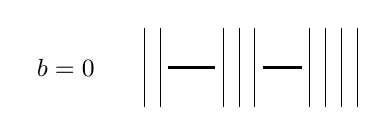
\begin{tikzpicture}
        
      \node at(0, .5)(a){\small{$b=0$}};
      \draw(1, 0) to (1, 1);
      \draw(1.2, 0) to (1.2, 1);
      \draw[line width = .3mm](1.3, .5) to (1.9, .5);
      \draw(2, 0) to (2, 1);
      \draw(2.2, 0) to(2.2, 1);
      \draw(2.4, 0) to (2.4, 1);
      \draw[line width = .3mm](2.5, .5) to (3, .5);
      \draw(3.1, 0) to (3.1, 1);
      \draw(3.3, 0) to (3.3, 1);
      \draw(3.5, 0) to (3.5, 1);
      \draw(3.7, 0) to (3.7, 1);
      \end{tikzpicture}}
  \end{minipage}
   \begin{minipage}{.45\textwidth}
   ~\centering
     ~\resizebox{.5\textwidth}{.1\textheight}{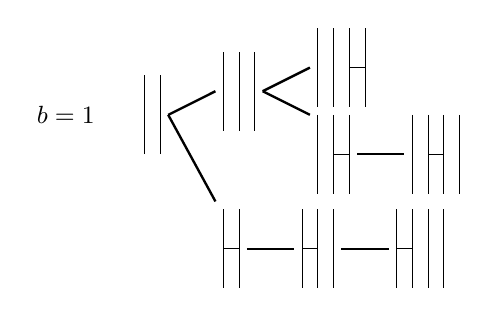
\begin{tikzpicture}
        
      \node at(0, .5)(a){\small{$b=1$}};
        \draw(1, 0) to (1, 1);
        \draw(1.2, 0) to (1.2, 1);
     \draw[line width = .3mm](1.3, .5) to (1.9, .8);
        \draw(2, .3) to (2, 1.3);
        \draw(2.2, .3) to(2.2, 1.3);
        \draw(2.4, .3) to (2.4, 1.3);
      \draw[line width = .3mm](2.5, .8) to (3.1, 1.1);
        \draw(3.2, 0.6) to (3.2, 1.6);
        \draw(3.4, 0.6) to (3.4, 1.6);
        \draw(3.6, 0.6) to (3.6, 1.6);
        \draw(3.6, 1.1) to (3.8, 1.1);
      \draw(3.8, 0.6) to (3.8, 1.6);

     \draw[line width = .3mm](2.5, .8) to (3.1, .5);
        \draw(3.2, .5) to (3.2, -.5);
        \draw(3.4, .5) to (3.4, -.5);
          \draw(3.4, 0) to (3.6, 0);                
        \draw(3.6, .5) to (3.6, -.5);


      \draw[line width = .3mm](3.7, 0) to (4.3, 0);
        \draw(4.4, .5) to (4.4, -.5);
        \draw(4.6, .5) to (4.6, -.5);
        \draw(4.8, .5) to (4.8, -.5);
                  \draw(4.6, 0) to (4.8, 0);                
        \draw(5, .5) to (5, -.5);


        \draw[line width= .3mm](1.3, .5) to (1.9, -.6);
          \draw(2, -.7) to (2, -1.7);
            \draw(2, -1.2) to (2.2, -1.2);
          \draw(2.2, -.7) to (2.2, -1.7);

        \draw[line width= .3mm](2.3, -1.2) to (2.9, -1.2);
        \draw(3, -.7) to (3, -1.7);
            \draw(3, -1.2) to (3.2, -1.2);
        \draw(3.2, -.7) to (3.2, -1.7);
        \draw(3.4, -.7) to (3.4, -1.7);
        \draw[line width= .3mm](3.5, -1.2) to (4.1, -1.2);
        \draw(4.2, -.7) to (4.2, -1.7);
            \draw(4.2, -1.2) to (4.4, -1.2);
        \draw(4.4, -.7) to (4.4, -1.7);
        \draw(4.6, -.7) to (4.6, -1.7);
        \draw(4.8, -.7) to (4.8, -1.7);
        




      \end{tikzpicture}}
      
    \end{minipage}
    \begin{minipage}{.45\textwidth}
     ~\centering
     ~\resizebox{.5\textwidth}{.2\textheight}{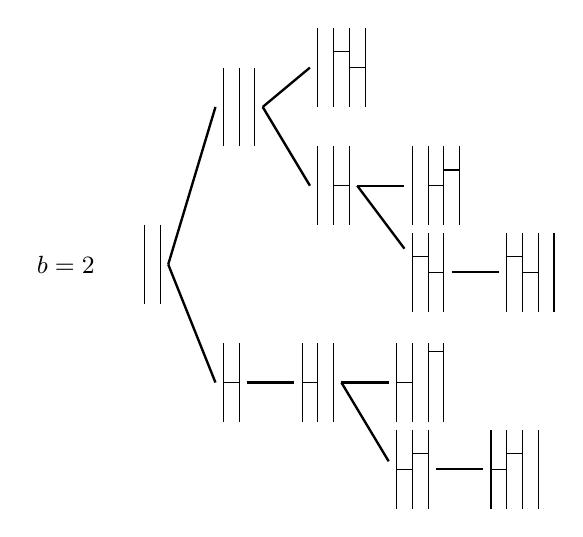
\begin{tikzpicture}
      \node at(0, 5.5){\small{$b=2$}};  
      %%t1
      \draw(1, 5) to (1, 6);
      \draw(1.2, 5) to (1.2, 6);
    \draw[line width = .3mm](1.3, 5.5) to (1.9, 7.5);
      \draw(2, 8) to (2, 7);
      \draw(2.2, 8) to (2.2, 7);
      \draw(2.4, 8) to (2.4, 7);
    \draw[line width = .3mm](2.5, 7.5) to (3.1, 8);
      \draw(3.2, 7.5) to (3.2, 8.5);
      \draw(3.4, 7.5) to (3.4, 8.5);
        \draw(3.4, 8.2) to (3.6, 8.2);
      \draw(3.6, 7.5) to (3.6, 8.5);
        \draw(3.6, 8) to (3.8, 8);
      \draw(3.8, 7.5) to (3.8, 8.5);

      %%tt2
    \draw[line width=.3mm](2.5, 7.5) to (3.1, 6.5);
      \draw(3.2, 7) to (3.2, 6);
      \draw(3.4, 7) to (3.4, 6);
        \draw(3.4, 6.5) to (3.6, 6.5);
      \draw(3.6, 7) to (3.6, 6);
    
    \draw[line width = .3mm](3.7, 6.5) to (4.3, 6.5);
      \draw(4.4, 6) to (4.4, 7);
      \draw(4.6, 6) to (4.6, 7);
        \draw(4.6, 6.5) to (4.8, 6.5);
      \draw(4.8, 6) to (4.8, 7);
        \draw(4.8, 6.7) to (5, 6.7);
      \draw(5, 6) to (5, 7);
    
    \draw[line width = .3mm](3.7, 6.5) to (4.3, 5.7);
      \draw(4.4, 5.9) to (4.4, 4.9);
        \draw(4.4, 5.6) to (4.6, 5.6);
      \draw(4.6, 5.9) to (4.6, 4.9);
        \draw(4.6, 5.4) to (4.8, 5.4);
      \draw(4.8, 5.9) to (4.8, 4.9);
    
   \draw[line width = .3mm](4.9, 5.4) to (5.5, 5.4);
      \draw(5.6, 5.9) to (5.6, 4.9);
        \draw(5.6, 5.6) to (5.8, 5.6);
      \draw(5.8, 5.9) to (5.8, 4.9);
        \draw(5.8, 5.4) to (6, 5.4);
      \draw(6, 5.9) to (6, 4.9);
      \draw(6.2, 5.9) to (6.2, 4.9);

    \draw[line width = .3mm](1.3, 5.5) to (1.9, 4);
    
        \draw(2, 4.5) to (2, 3.5);
          \draw(2, 4) to (2.2, 4);
        \draw(2.2, 4.5) to (2.2, 3.5);

    \draw[line width = .3mm](2.3, 4) to (2.9, 4);
        \draw(3, 4.5) to (3, 3.5);
          \draw(3, 4) to (3.2, 4);
        \draw(3.2, 4.5) to (3.2, 3.5);
        \draw(3.4, 4.5) to (3.4, 3.5);
    \draw[line width = .3mm](3.5, 4) to (4.1, 4);
    \draw[line width = .3mm](3.5, 4) to (4.1, 3);
      \draw(4.2, 4.5) to (4.2, 3.5);
        \draw(4.2, 4) to (4.4, 4);
      \draw(4.4, 4.5) to (4.4, 3.5);
      \draw(4.6, 4.5) to (4.6, 3.5);
        \draw(4.6, 4.4) to (4.8, 4.4);
      \draw(4.8, 4.5) to (4.8, 3.5);

      \draw(4.2, 3.4) to (4.2, 2.4);
        \draw(4.2, 2.9) to (4.4, 2.9);
      \draw(4.4, 3.4) to (4.4, 2.4);
        \draw(4.4, 3.1) to (4.6, 3.1);
      \draw(4.6, 3.4) to (4.6, 2.4);
    
    \draw[line width = .3mm](4.7, 2.9) to (5.3, 2.9);
        \draw(5.4, 3.4) to (5.4, 2.4);
          \draw(5.4, 2.9) to (5.6, 2.9);
        \draw(5.6, 3.4) to (5.6, 2.4);
          \draw(5.6, 3.1) to (5.8, 3.1);
        \draw(5.8, 3.4) to (5.8, 2.4);
        \draw(6.0, 3.4) to (6.0, 2.4);




    \end{tikzpicture}}
  \end{minipage}
  \begin{minipage}{.45\textwidth}
   ~\centering
   ~\resizebox{.5\textwidth}{.25\textheight}{\begin{tikzpicture}
      \node at(0, 5.5){\small{$b=3$}};
        %%t1
        \draw(1, 5) to (1, 6);
        \draw(1.2, 5) to (1.2, 6);
      \draw[line width = .3mm](1.3, 5.5) to (1.9, 7.5);
        \draw(2, 7) to (2, 8);
        \draw(2.2, 7) to (2.2, 8);
        \draw(2.4, 7) to (2.4, 8);
      \draw[line width = .3mm](2.5, 7.5) to (2.9, 9);
      \draw[line width = .3mm](2.5, 7.5) to (2.9, 6.5);
        %%Leaf1
        \draw(3, 9.5) to (3, 8.5);
          \draw(3, 9.4) to (3.2, 9.4);
        \draw(3.2, 9.5) to (3.2, 8.5);
          \draw(3.2, 9.2) to (3.4, 9.2);
        \draw(3.4, 9.5) to (3.4, 8.5);
          \draw(3.4, 9) to (3.6, 9);
        \draw(3.6, 9.5) to (3.6, 8.5);
        %%t2
        \draw(3, 7) to (3, 6);
        \draw(3.2, 7) to (3.2, 6);
          \draw(3.2, 6.5) to (3.4, 6.5);
        \draw(3.4, 7) to (3.4, 6);
        \draw[line width = .3mm](3.5, 6.5) to (4.1, 6.5);
        \draw[line width = .3mm](3.5, 6.5) to (4.1, 5.5);
        %%Leaf2
        \draw(4.2, 6) to (4.2, 7);
        \draw(4.4, 6) to (4.4, 7);
          \draw(4.4, 6.7) to (4.6, 6.7);
          \draw(4.4, 6.3) to (4.6, 6.3);
        \draw(4.6, 6) to (4.6, 7);
          \draw(4.6, 6.5) to (4.8, 6.5);
        \draw(4.8, 6) to (4.8, 7);

        \draw(4.2, 5.9) to (4.2, 4.9);
          \draw(4.2, 5.5) to (4.4, 5.5);
        \draw(4.4, 5.9) to (4.4, 4.9);
          \draw(4.4, 5.3) to (4.6, 5.3);
        \draw(4.6, 5.9) to (4.6, 4.9);
      \draw[line width = .3mm](4.7, 5.4) to (5.3, 5.4);
      %%leaf 3
        \draw(5.4, 4.9) to (5.4, 5.9);
          \draw(5.4, 5.5)to(5.6, 5.5);
        \draw(5.6, 4.9) to (5.6, 5.9);
          \draw(5.6, 5.3) to (5.8, 5.3);
        \draw(5.8, 4.9) to (5.8, 5.9);
          \draw(5.8, 5.5)to(6, 5.5);
        \draw(6.0, 4.9) to (6.0, 5.9);

      %%Line
      \draw[line width=.3mm](1.3, 5.5) to (1.9, 4);

        \draw(2, 4.5) to (2, 3.5);
          \draw(2, 3.6) to (2.2, 3.6);
        \draw(2.2, 4.5) to (2.2, 3.5);

      \draw[line width = .3mm](2.3, 4) to (2.9, 4);
        \draw(3.0, 4.5) to (3.0, 3.5);
          \draw(3, 3.6) to (3.2, 3.6);
        \draw(3.2, 4.5) to (3.2, 3.5);
      
        \draw(3.4, 4.5) to (3.4, 3.5);
      
        \draw[line width = .3mm](3.5, 4) to (4.1, 4.3);
      %%leaf 4
        \draw(4.2, 3.8) to (4.2, 4.8);
          \draw(4.2, 3.9) to (4.4, 3.9);
        \draw(4.4, 3.8) to (4.4, 4.8);
          \draw(4.4, 4.5) to (4.6, 4.5);
        \draw(4.6, 3.8) to (4.6, 4.8);
          \draw(4.6, 4.3) to (4.8, 4.3);
        \draw(4.8, 3.8) to (4.8, 4.8);

    \draw[line width = .3mm](3.5, 4) to (4.1, 3.5);
      \draw(4.2, 3.7) to (4.2, 2.7);
        \draw(4.2,  2.8) to (4.4, 2.8);
      \draw(4.4, 3.7) to (4.4, 2.7);
        \draw(4.4, 3) to (4.6, 3);
      \draw(4.6, 3.7) to (4.6, 2.7);

    \draw[line width = .3mm](4.7, 3.2) to (5.3, 3.9);
    %%leaf 5
      \draw(5.4, 4.4) to (5.4, 3.4);
        \draw(5.4, 3.5) to (5.6, 3.5);
        \draw(5.6, 3.7) to (5.8, 3.7);
        \draw(5.8, 3.9) to (6.0, 3.9);
      \draw(5.6, 4.4) to (5.6, 3.4);
      \draw(5.8, 4.4) to (5.8, 3.4);
      \draw(6.0, 4.4) to (6.0, 3.4);
   
    \draw[line width = .3mm](4.7, 3.2) to (5.3, 2.5);
    \draw(5.4, 3) to (5.4, 2);
      \draw(5.4, 2.1) to (5.6, 2.1);
      \draw(5.4, 2.5) to (5.6, 2.5);
    \draw(5.6, 3) to (5.6, 2);
      \draw(5.6, 2.3) to (5.8, 2.3);
    \draw(5.8, 3) to (5.8, 2);

    \draw[line width = .3mm](5.9, 2.5) to (6.4, 2.5);
    \draw(6.5, 3) to (6.5, 2);
      \draw(6.5, 2.1) to (6.7, 2.1);
      \draw(6.5, 2.5) to (6.7, 2.5);
    \draw(6.7, 3) to (6.7, 2);
      \draw(6.7, 2.3) to (6.9, 2.3);
    \draw(6.9, 3) to (6.9, 2);
    \draw(7.1, 3) to (7.1, 2);




    \end{tikzpicture}}
  \end{minipage}
   \begin{minipage}{.45\textwidth}
   ~\centering
   ~\resizebox{.5\textwidth}{.25\textheight}{\begin{tikzpicture}
      \node at(0, 5.5){\small{$b=4$}};
        %%t1
        \draw(1, 5) to (1, 6);
        \draw(1.2, 5) to (1.2, 6);
      \draw[line width = .3mm](1.3, 5.5) to (1.9, 7.5);
        \draw(2, 7) to (2, 8);
        \draw(2.2, 7) to (2.2, 8);
        \draw(2.4, 7) to (2.4, 8);
      \draw[line width = .3mm](2.5, 7.5) to (2.9, 9);
      \draw[line width = .3mm](2.5, 7.5) to (2.9, 7.5);
        %%Leaf1
        \draw(3, 9.5) to (3, 8.5);
          \draw(3, 9.4) to (3.2, 9.4);
        \draw(3.2, 9.5) to (3.2, 8.5);
          \draw(3.2, 9.2) to (3.4, 9.2);
        \draw(3.4, 9.5) to (3.4, 8.5);
          \draw(3.4, 9) to (3.6, 9);
        \draw(3.6, 9.5) to (3.6, 8.5);
        %%t2
        \draw(3, 7) to (3, 8);
        \draw(3.2, 7) to (3.2, 8);
          \draw(3.2, 7.5) to (3.4, 7.5);
        \draw(3.4, 7) to (3.4, 8);
        \draw[line width = .3mm](3.5, 7.5) to (4.1, 7.5);
        %%Leaf2
        \draw(4.2, 7) to (4.2, 8);
          \draw(4.2, 7.9) to (4.4, 7.9);
        \draw(4.4, 7) to (4.4, 8);
          \draw(4.4, 7.3) to (4.6, 7.3);
          \draw(4.4, 7.7) to (4.6, 7.7);
        \draw(4.6, 7) to (4.6, 8);
          \draw(4.6, 7.5) to (4.8, 7.5);s
        \draw(4.8, 7) to (4.8, 8);
        %%\draw[line width = .3mm](3.5, 6.5) to (4.1, 5.5);

        \draw[line width = .3mm](3.5, 7.5) to (4.1, 6.5);

        \draw(4.2, 6.9) to (4.2, 5.9);
          \draw(4.2, 6.4) to (4.4, 6.4);
        \draw(4.4, 6.9) to (4.4, 5.9);
          \draw(4.4, 6.2) to (4.6, 6.2);
        \draw(4.6, 6.9) to (4.6, 5.9);

        \draw[line width = .3mm](4.7, 6.4) to (5.3, 6.4);
      %%leaf 3
        \draw(5.4, 6.9) to (5.4, 5.9);
          \draw(5.4, 6.4) to (5.6, 6.4);
        \draw(5.6, 6.9) to (5.6, 5.9);
          \draw(5.6, 6.2) to (5.8, 6.2);
          \draw(5.6, 6.6) to (5.8, 6.6);
        \draw(5.8, 6.9) to (5.8, 5.9);
          \draw(5.8, 6.4) to (6.0, 6.4);
        \draw(6.0, 6.9) to (6.0, 5.9);


      \draw[line width = .3mm](1.3, 5.5) to (1.9, 3.5);
      \draw(1.9, 4) to (1.9, 3);
        \draw(1.9, 3.1) to (2.1, 3.1);
      \draw(2.1, 4) to (2.1, 3);

      \draw[line width = .3mm](2.2, 3.5) to (2.8, 4.1);
      
      \draw(2.9, 4.6) to (2.9, 3.6);
        \draw(2.9, 3.7) to (3.1, 3.7);
      \draw(3.1, 4.6) to (3.1, 3.6);
      \draw(3.3, 4.6) to (3.3, 3.6);

      \draw[line width = .3mm](3.4, 4.1) to (4,5.1);
      %%Leaf 4
      \draw(4.1, 5.6) to (4.1, 4.6);
        \draw(4.1, 4.7) to (4.3, 4.7);
        \draw(4.1, 5.5) to (4.3, 5.5);
      \draw(4.3, 4.6) to (4.3, 5.6);
        \draw(4.3, 5.3) to (4.5, 5.3);
      \draw(4.5, 4.6) to (4.5, 5.6);
        \draw(4.5, 5.1) to (4.7, 5.1);
      \draw(4.7, 4.6) to (4.7, 5.6);

      \draw[line width = .3mm](3.4, 4.1) to (4,3.1);
      \draw(4.1, 3.6) to (4.1, 2.6);
        \draw(4.1, 2.7) to (4.3, 2.7);
      \draw(4.3, 3.6) to (4.3, 2.6);
        \draw(4.3, 2.9) to (4.5, 2.9);
      \draw(4.5, 3.6) to (4.5, 2.6);

      \draw[line width = .3mm](4.6, 3.1) to (5.2, 3.8);
      %%leaf 5
      \draw(5.3, 4.3) to (5.3, 3.3);
        \draw(5.3, 3.4) to (5.5, 3.4);
      \draw(5.5, 4.3) to (5.5, 3.3);
        \draw(5.5, 3.6) to (5.7, 3.6);
      \draw(5.7, 4.3) to (5.7, 3.3);
        \draw(5.7, 3.8) to (5.9, 3.8);
        \draw(5.5, 4) to (5.7, 4);
      \draw(5.9, 4.3) to (5.9, 3.3);
      
      
      \draw[line width = .3mm](4.6, 3.1) to (5.2, 2.5);

      \draw(5.3, 3) to (5.3, 2);
        \draw(5.3, 2.1) to (5.5, 2.1);
        \draw(5.3, 2.5) to (5.5, 2.5);
      \draw(5.5, 3) to (5.5, 2);
        \draw(5.5, 2.3) to (5.7, 2.3);
      \draw(5.7, 3) to (5.7, 2);

      \draw[line width = .3mm](5.8, 2.5) to (6.4, 2.5);

      
      \draw(6.5, 3) to (6.5, 2);
        \draw(6.5, 2.1) to (6.7, 2.1);
        \draw(6.5, 2.5) to (6.7, 2.5);
      \draw(6.7, 3) to (6.7, 2);
        \draw(6.7, 2.3) to (6.9, 2.3);
      \draw(6.9, 3) to (6.9, 2);
        \draw(6.9, 2.5) to (7.1, 2.5);
      \draw(7.1, 2) to (7.1, 3);






    \end{tikzpicture}}
  \end{minipage}
  \begin{minipage}{.45\textwidth}
   ~\centering
   ~\resizebox{.5\textwidth}{.25\textheight}{\begin{tikzpicture}
      \node at(0, 5.5){\small{$b=5$}};
        %%t1
        \draw(1, 5) to (1, 6);
        \draw(1.2, 5) to (1.2, 6);
      \draw[line width = .3mm](1.3, 5.5) to (1.9, 7.5);
        \draw(2, 7) to (2, 8);
        \draw(2.2, 7) to (2.2, 8);
        \draw(2.4, 7) to (2.4, 8);
      \draw[line width = .3mm](2.5, 7.5) to (2.9, 9);
      \draw[line width = .3mm](2.5, 7.5) to (2.9, 7.5);
        %%Leaf1
        \draw(3, 9.5) to (3, 8.5);
          \draw(3, 9.4) to (3.2, 9.4);
        \draw(3.2, 9.5) to (3.2, 8.5);
          \draw(3.2, 9.2) to (3.4, 9.2);
        \draw(3.4, 9.5) to (3.4, 8.5);
          \draw(3.4, 9) to (3.6, 9);
        \draw(3.6, 9.5) to (3.6, 8.5);
        %%t2
        \draw(3, 7) to (3, 8);
        \draw(3.2, 7) to (3.2, 8);
          \draw(3.2, 7.5) to (3.4, 7.5);
        \draw(3.4, 7) to (3.4, 8);
        \draw[line width = .3mm](3.5, 7.5) to (4.1, 7.5);
        %%Leaf2
        \draw(4.2, 7) to (4.2, 8);
          \draw(4.2, 7.9) to (4.4, 7.9);
        \draw(4.4, 7) to (4.4, 8);
          \draw(4.4, 7.3) to (4.6, 7.3);
          \draw(4.4, 7.7) to (4.6, 7.7);
        \draw(4.6, 7) to (4.6, 8);
          \draw(4.6, 7.5) to (4.8, 7.5);
        \draw(4.8, 7) to (4.8, 8);
        \draw[line width = .3mm](3.5, 7.5) to (4.1, 6.5);

        \draw[line width = .3mm](3.5, 7.5) to (4.1, 6.5);

        \draw(4.2, 6.9) to (4.2, 5.9);
          \draw(4.2, 6.4) to (4.4, 6.4);
        \draw(4.4, 6.9) to (4.4, 5.9);
          \draw(4.4, 6.2) to (4.6, 6.2);
        \draw(4.6, 6.9) to (4.6, 5.9);

        \draw[line width = .3mm](4.7, 6.4) to (5.3, 6.4);
      %%leaf 3
        \draw(5.4, 6.9) to (5.4, 5.9);
          \draw(5.4, 6.4) to (5.6, 6.4);
          \draw(5.4, 6.8) to (5.6, 6.8);
        \draw(5.6, 6.9) to (5.6, 5.9);
          \draw(5.6, 6.2) to (5.8, 6.2);
          \draw(5.6, 6.6) to (5.8, 6.6);
        \draw(5.8, 6.9) to (5.8, 5.9);
          \draw(5.8, 6.4) to (6.0, 6.4);
        \draw(6.0, 6.9) to (6.0, 5.9);


      \draw[line width = .3mm](1.3, 5.5) to (1.9, 3.5);
      \draw(1.9, 4) to (1.9, 3);
        \draw(1.9, 3.1) to (2.1, 3.1);
      \draw(2.1, 4) to (2.1, 3);

      \draw[line width = .3mm](2.2, 3.5) to (2.8, 4.1);
      
      \draw(2.9, 4.6) to (2.9, 3.6);
        \draw(2.9, 3.7) to (3.1, 3.7);
      \draw(3.1, 4.6) to (3.1, 3.6);
      \draw(3.3, 4.6) to (3.3, 3.6);

      \draw[line width = .3mm](3.4, 4.1) to (4,5.1);
      %%Leaf 4
      \draw(4.1, 5.6) to (4.1, 4.6);
        \draw(4.1, 4.7) to (4.3, 4.7);
        \draw(4.1, 5.5) to (4.3, 5.5);
      \draw(4.3, 4.6) to (4.3, 5.6);
        \draw(4.3, 5.3) to (4.5, 5.3);
      \draw(4.5, 4.6) to (4.5, 5.6);
        \draw(4.5, 5.1) to (4.7, 5.1);
      \draw(4.7, 4.6) to (4.7, 5.6);

      \draw[line width = .3mm](3.4, 4.1) to (4,3.1);
      \draw(4.1, 3.6) to (4.1, 2.6);
        \draw(4.1, 2.7) to (4.3, 2.7);
      \draw(4.3, 3.6) to (4.3, 2.6);
        \draw(4.3, 2.9) to (4.5, 2.9);
      \draw(4.5, 3.6) to (4.5, 2.6);

      \draw[line width = .3mm](4.6, 3.1) to (5.2, 3.8);
      %%leaf 5
      \draw(5.3, 4.3) to (5.3, 3.3);
        \draw(5.3, 3.4) to (5.5, 3.4);
        \draw(5.3, 4.2) to (5.5, 4.2);

      \draw(5.5, 4.3) to (5.5, 3.3);
        \draw(5.5, 3.6) to (5.7, 3.6);
      \draw(5.7, 4.3) to (5.7, 3.3);
        \draw(5.7, 3.8) to (5.9, 3.8);
        \draw(5.5, 4) to (5.7, 4);
      \draw(5.9, 4.3) to (5.9, 3.3);
      
      
      \draw[line width = .3mm](4.6, 3.1) to (5.2, 2.5);

      \draw(5.3, 3) to (5.3, 2);
        \draw(5.3, 2.1) to (5.5, 2.1);
        \draw(5.3, 2.5) to (5.5, 2.5);
      \draw(5.5, 3) to (5.5, 2);
        \draw(5.5, 2.3) to (5.7, 2.3);
      \draw(5.7, 3) to (5.7, 2);

      \draw[line width = .3mm](5.8, 2.5) to (6.4, 2.5);

      
      \draw(6.5, 3) to (6.5, 2);
        \draw(6.5, 2.1) to (6.7, 2.1);
        \draw(6.5, 2.5) to (6.7, 2.5);
      \draw(6.7, 3) to (6.7, 2);
        \draw(6.7, 2.3) to (6.9, 2.3);
        \draw(6.7, 2.7) to (6.9, 2.7);
      \draw(6.9, 3) to (6.9, 2);
        \draw(6.9, 2.5) to (7.1, 2.5);
      \draw(7.1, 2) to (7.1, 3);






    \end{tikzpicture}}
  \end{minipage}
   \begin{minipage}{.45\textwidth}
   ~\centering
   ~\resizebox{.5\textwidth}{.25\textheight}{\begin{tikzpicture}
      \node at(0, 5.5){\small{$b=6$}};
        %%t1
        \draw(1, 5) to (1, 6);
        \draw(1.2, 5) to (1.2, 6);
      \draw[line width = .3mm](1.3, 5.5) to (1.9, 7.5);
        \draw(2, 7) to (2, 8);
        \draw(2.2, 7) to (2.2, 8);
        \draw(2.4, 7) to (2.4, 8);
      \draw[line width = .3mm](2.5, 7.5) to (2.9, 9);
      \draw[line width = .3mm](2.5, 7.5) to (2.9, 7.5);
        %%Leaf1
        \draw(3, 9.5) to (3, 8.5);
          \draw(3, 9.4) to (3.2, 9.4);
        \draw(3.2, 9.5) to (3.2, 8.5);
          \draw(3.2, 9.2) to (3.4, 9.2);
        \draw(3.4, 9.5) to (3.4, 8.5);
          \draw(3.4, 9) to (3.6, 9);
        \draw(3.6, 9.5) to (3.6, 8.5);
        %%t2
        \draw(3, 7) to (3, 8);
        \draw(3.2, 7) to (3.2, 8);
          \draw(3.2, 7.5) to (3.4, 7.5);
        \draw(3.4, 7) to (3.4, 8);
        \draw[line width = .3mm](3.5, 7.5) to (4.1, 7.5);
        %%Leaf2
        \draw(4.2, 7) to (4.2, 8);
          \draw(4.2, 7.9) to (4.4, 7.9);
        \draw(4.4, 7) to (4.4, 8);
          \draw(4.4, 7.3) to (4.6, 7.3);
          \draw(4.4, 7.7) to (4.6, 7.7);
        \draw(4.6, 7) to (4.6, 8);
          \draw(4.6, 7.5) to (4.8, 7.5);
        \draw(4.8, 7) to (4.8, 8);
        \draw[line width = .3mm](3.5, 7.5) to (4.1, 6.5);

        \draw[line width = .3mm](3.5, 7.5) to (4.1, 6.5);

        \draw(4.2, 6.9) to (4.2, 5.9);
          \draw(4.2, 6.4) to (4.4, 6.4);
        \draw(4.4, 6.9) to (4.4, 5.9);
          \draw(4.4, 6.2) to (4.6, 6.2);
        \draw(4.6, 6.9) to (4.6, 5.9);

        \draw[line width = .3mm](4.7, 6.4) to (5.3, 6.4);
      %%leaf 3
        \draw(5.4, 6.9) to (5.4, 5.9);
          \draw(5.4, 6.4) to (5.6, 6.4);
          \draw(5.4, 6.8) to (5.6, 6.8);
        \draw(5.6, 6.9) to (5.6, 5.9);
          \draw(5.6, 6.2) to (5.8, 6.2);
          \draw(5.6, 6.6) to (5.8, 6.6);
        \draw(5.8, 6.9) to (5.8, 5.9);
          \draw(5.8, 6.4) to (6.0, 6.4);
        \draw(6.0, 6.9) to (6.0, 5.9);


      \draw[line width = .3mm](1.3, 5.5) to (1.9, 3.5);
      \draw(1.9, 4) to (1.9, 3);
        \draw(1.9, 3.1) to (2.1, 3.1);
      \draw(2.1, 4) to (2.1, 3);

      \draw[line width = .3mm](2.2, 3.5) to (2.8, 4.1);
      
      \draw(2.9, 4.6) to (2.9, 3.6);
        \draw(2.9, 3.7) to (3.1, 3.7);
      \draw(3.1, 4.6) to (3.1, 3.6);
      \draw(3.3, 4.6) to (3.3, 3.6);

      \draw[line width = .3mm](3.4, 4.1) to (4,5.1);
      %%Leaf 4
      \draw(4.1, 5.6) to (4.1, 4.6);
        \draw(4.1, 4.7) to (4.3, 4.7);
        \draw(4.1, 5.5) to (4.3, 5.5);
      \draw(4.3, 4.6) to (4.3, 5.6);
        \draw(4.3, 5.3) to (4.5, 5.3);
      \draw(4.5, 4.6) to (4.5, 5.6);
        \draw(4.5, 5.1) to (4.7, 5.1);
      \draw(4.7, 4.6) to (4.7, 5.6);

      \draw[line width = .3mm](3.4, 4.1) to (4,3.1);
      \draw(4.1, 3.6) to (4.1, 2.6);
        \draw(4.1, 2.7) to (4.3, 2.7);
      \draw(4.3, 3.6) to (4.3, 2.6);
        \draw(4.3, 2.9) to (4.5, 2.9);
      \draw(4.5, 3.6) to (4.5, 2.6);

      \draw[line width = .3mm](4.6, 3.1) to (5.2, 3.8);
      %%leaf 5
      \draw(5.3, 4.3) to (5.3, 3.3);
        \draw(5.3, 3.4) to (5.5, 3.4);
        \draw(5.3, 4.2) to (5.5, 4.2);

      \draw(5.5, 4.3) to (5.5, 3.3);
        \draw(5.5, 3.6) to (5.7, 3.6);
      \draw(5.7, 4.3) to (5.7, 3.3);
        \draw(5.7, 3.8) to (5.9, 3.8);
        \draw(5.5, 4) to (5.7, 4);
      \draw(5.9, 4.3) to (5.9, 3.3);
      
      
      \draw[line width = .3mm](4.6, 3.1) to (5.2, 2.5);

      \draw(5.3, 3) to (5.3, 2);
        \draw(5.3, 2.1) to (5.5, 2.1);
        \draw(5.3, 2.5) to (5.5, 2.5);
      \draw(5.5, 3) to (5.5, 2);
        \draw(5.5, 2.3) to (5.7, 2.3);
      \draw(5.7, 3) to (5.7, 2);

      \draw[line width = .3mm](5.8, 2.5) to (6.4, 2.5);

      
      \draw(6.5, 3) to (6.5, 2);
        \draw(6.5, 2.1) to (6.7, 2.1);
        \draw(6.5, 2.5) to (6.7, 2.5);
      \draw(6.7, 3) to (6.7, 2);
        \draw(6.7, 2.3) to (6.9, 2.3);
        \draw(6.7, 2.7) to (6.9, 2.7);
      \draw(6.9, 3) to (6.9, 2);
        \draw(6.9, 2.5) to (7.1, 2.5);
        \draw(6.9, 2.9) to (7.1, 2.9);
      \draw(7.1, 2) to (7.1, 3);






    \end{tikzpicture}}
  \end{minipage}
  
  

     
  \caption{The forest for all ladders in $L_{4}$ generated by the Cyclic Bar Algorithm. The leaf nodes present a possibly correct candidate ladder. 
  If the ladder in the leaf has enough bars, then it is a legitimate ladder in the tree.}
  \label{Fig:CanLForest}
\end{figure}
\end{center}
It has been stated that the forest produced by the Cyclic Bar algorithm generates
$L_{n}$. This claim will be proven below.


\begin{theorem}
  The forest produced by {\sc CyclicBar} generates $L_{n}$
\end{theorem}


\begin{proof}
  The proof is done by way of a combinatorial proof and induction. Rather than list ladders, we shall list permutations using the same method.  
  Let $List(n, k)$ be the listing of permutations of order $n$ with $k$ inversions. The hypothesis is that $List(n, k)=\sum_{m=0}^{k} List(n-1, m)$ 
  given $n>1$ and $k \geq 0$.
  The base case is $n=2$ and $k=0$. We know that the identity permutation of order $1$ has no inversions. We know that the list containing the identity 
  permutation of order $1$ is of length one. We know that the list containing the identity permutation of order $2$ is of length one. By appending the 
  value $2$ to the only permutation in the list $List(1, 0)$ we get the only permutation in the list $List(2, 0)$. Therefore the base case checks out.
  
  Suppose we have the list of permutations for $List(n-1, 0) \dots List(n-1, k)$. We want to show that we can insert the $nth$ element into each of the
  permutations in each of these lists such that the resulting permutations have $n$ elements with $k$ inversions. Partition $k$ into $k'$ and $k''$. Note that 
  $k'+k''=k$.
  Let $k'$ equal the number of inversions formed by the $nth$ element. Let $k''$ equal the number of elements not formed by the $nth$ element.
  We can look at the $List(n-1, 0) \dots List(n-1, k)$ as lists of permutations with $k''$ inversions. So we write 
  $List(n-1, 0) \dots List(n-1, k)$ as $List(n-1, k''=0) \dots List(n-1, k''=k)$. When $k''=0$ we know $List(n-1, 0)$ has one permutation, thus $k'=k$.
  The $nth$ element must be positioned $k'$ positions to the left of the $nth$ position in this one permutation from $List(n-1, 0)$ to form a permutation of order $n$ with $k$ inversions. 
  In general, we can say that for each of the permutations from each of the $List(n-1, k'')$, we know that the $nth$ element must be positioned $k-k''$ to the left of the $nth$ position in order to 
  ce a permutation of length $n$ with $k$ inversions. Thus, by exhaustively inserting the $nth$ element in all $k-k''=k'$ positions to the left of the $nth$ position 
  in all permutations from all $List(n-1, k'')$, we get all permutations of order $n$ with $k$ inversions. 
  Therefore $List(n, k) = List(n, k') + \sum_{k''=0}^{k} List(n-1, k'') $.
  Seeing as an inversion in a permutation corresponds to a bar in 
  a ladder, then by using this same proof on ladders, we can generate all ladders with $k$ bars. 
  Which is to say that $ladders(n, k) = Ladders(n, k') + \sum_{k''=0}^{k} Ladders(n-1, k'')$.
  In order to list $L_{n}$ simply apply this same logic for all $k$ bars for $0 \leq k \leq n(n-1)/2$. To see an example of the above proof for $List(4, 2)$ refer to Table~\ref{Table:List4,2}.

\end{proof}

\begin{table}
  \begin{tabular}{|p{2cm}||p{2cm}||p{2cm}||p{2cm} ||p{2cm} ||p{2cm}||}
     \hline
        \small{$n$ value}& \small{$k$ value} & \small{$k''$ value} & \small{$k'$ value} &\small{$L($n-1$, k'')$} & \small{$L(n, k)$}\\
        \hline
        \small{$4$} & \small{$2$} & \small{$0$} & \small{$2$} & \small{$(1,2,3)$} & \small{$(1,4,2,3)$} \\
        \hline
        \small{$4$} & \small{$2$} & \small{$1$} & \small{$1$} & \small{$(1,3,2)$} & \small{$(1,3,4,2)$} \\
        \small{$4$} & \small{$2$} & \small{$1$} & \small{$1$} & \small{$(2,1,3)$} & \small{$(2,1,4,3)$} \\
        \hline
        \small{$4$} & \small{$2$} & \small{$2$} & \small{$0$} & \small{$(3,1,2)$} & \small{$(3,1,2,4)$} \\                
        \small{$4$} & \small{$2$} & \small{$2$} & \small{$0$} & \small{$(2,3,1)$} & \small{$(2,3,1,4)$} \\
        \hline
  \end{tabular}
  \caption{The table showing all $List(4, 2)$ derived from $List(3, 0) \dots List(3, 2) + List(4, k')$}
  \label{Table:List4,2}
\end{table}


